% ==============================================================================
% Sustentación: Taller 2 - Redes Neuronales Multicapa (MLP) y Backpropagation
% Inteligencia Computacional Aplicada
% Maestría en Ciencias de la Información y las Comunicaciones (MCIC)
% Universidad Distrital Francisco José de Caldas
% ==============================================================================
\documentclass[aspectratio=169,10pt]{beamer}

\usepackage{fontspec}
\usepackage{graphicx}
\usepackage{tikz}
\usepackage{xcolor}
\usepackage{booktabs}
\usepackage{array}
\usepackage{amsmath,amssymb}
\usetikzlibrary{calc,positioning,shapes.geometric,arrows.meta,shadows,fit}

% ------------------------------------------------------------------------------
% Tipografía Institucional Oficial (Manual de Identidad Institucional UD)
% ------------------------------------------------------------------------------
\newfontfamily\cambriafont{cambria.ttc}[
  Path = assets/fonts/,
  BoldFont = cambriab.ttf,
  ItalicFont = cambriai.ttf,
  BoldItalicFont = cambriaz.ttf
]

\setsansfont{times.ttf}[
  Path = assets/fonts/,
  BoldFont = timesbd.ttf,
  ItalicFont = timesi.ttf,
  BoldItalicFont = timesbi.ttf
]
\setmainfont{times.ttf}[
  Path = assets/fonts/,
  BoldFont = timesbd.ttf,
  ItalicFont = timesi.ttf,
  BoldItalicFont = timesbi.ttf
]

% ------------------------------------------------------------------------------
% Paleta de Colores Oficial de la Universidad Distrital
% ------------------------------------------------------------------------------
\definecolor{UDRed}{HTML}{ED3237}       % Rojo gules institucional
\definecolor{UDDarkRed}{HTML}{B71C1C}   % Rojo oscuro contraste
\definecolor{UDGold}{HTML}{B49739}      % Dorado institucional
\definecolor{UDBlue}{HTML}{1291C0}      % Azul azur
\definecolor{UDGreen}{HTML}{00A859}     % Verde sinople
\definecolor{UDDarkGreen}{HTML}{047857} % Verde oscuro
\definecolor{UDSilver}{HTML}{64748B}    % Gris pizarra
\definecolor{UDSable}{HTML}{1E293B}     % Carbón texto
\definecolor{UDLightGray}{HTML}{F8FAFC} % Fondo de tarjetas
\definecolor{UDBorder}{HTML}{CBD5E1}    % Borde suave

% ------------------------------------------------------------------------------
% Configuración de Márgenes y Estilos Beamer
% ------------------------------------------------------------------------------
\setbeamertemplate{navigation symbols}{}
\setbeamersize{text margin left=3.15cm, text margin right=0.75cm}
\setbeamercolor{normal text}{fg=UDSable}

\setbeamertemplate{frametitle}{
  \vspace{0.45cm}
  \begin{minipage}{\textwidth}
    {\cambriafont\fontsize{12.5pt}{14.5pt}\bfseries\color{UDSable}\insertframetitle\par}
    \ifx\insertframesubtitle\@empty\else
      \vskip2pt
      {\cambriafont\fontsize{7.8pt}{9.5pt}\bfseries\color{UDRed}\insertframesubtitle\par}
    \fi
  \end{minipage}
}

\setbeamertemplate{footline}{
  \ifnum\thepage>1
    \hfill{\color{UDSilver}\fontsize{7pt}{8pt}\selectfont \insertframenumber\,/\,\inserttotalframenumber}\hspace{0.75cm}\vspace{0.35cm}
  \fi
}

\setbeamertemplate{background}{
  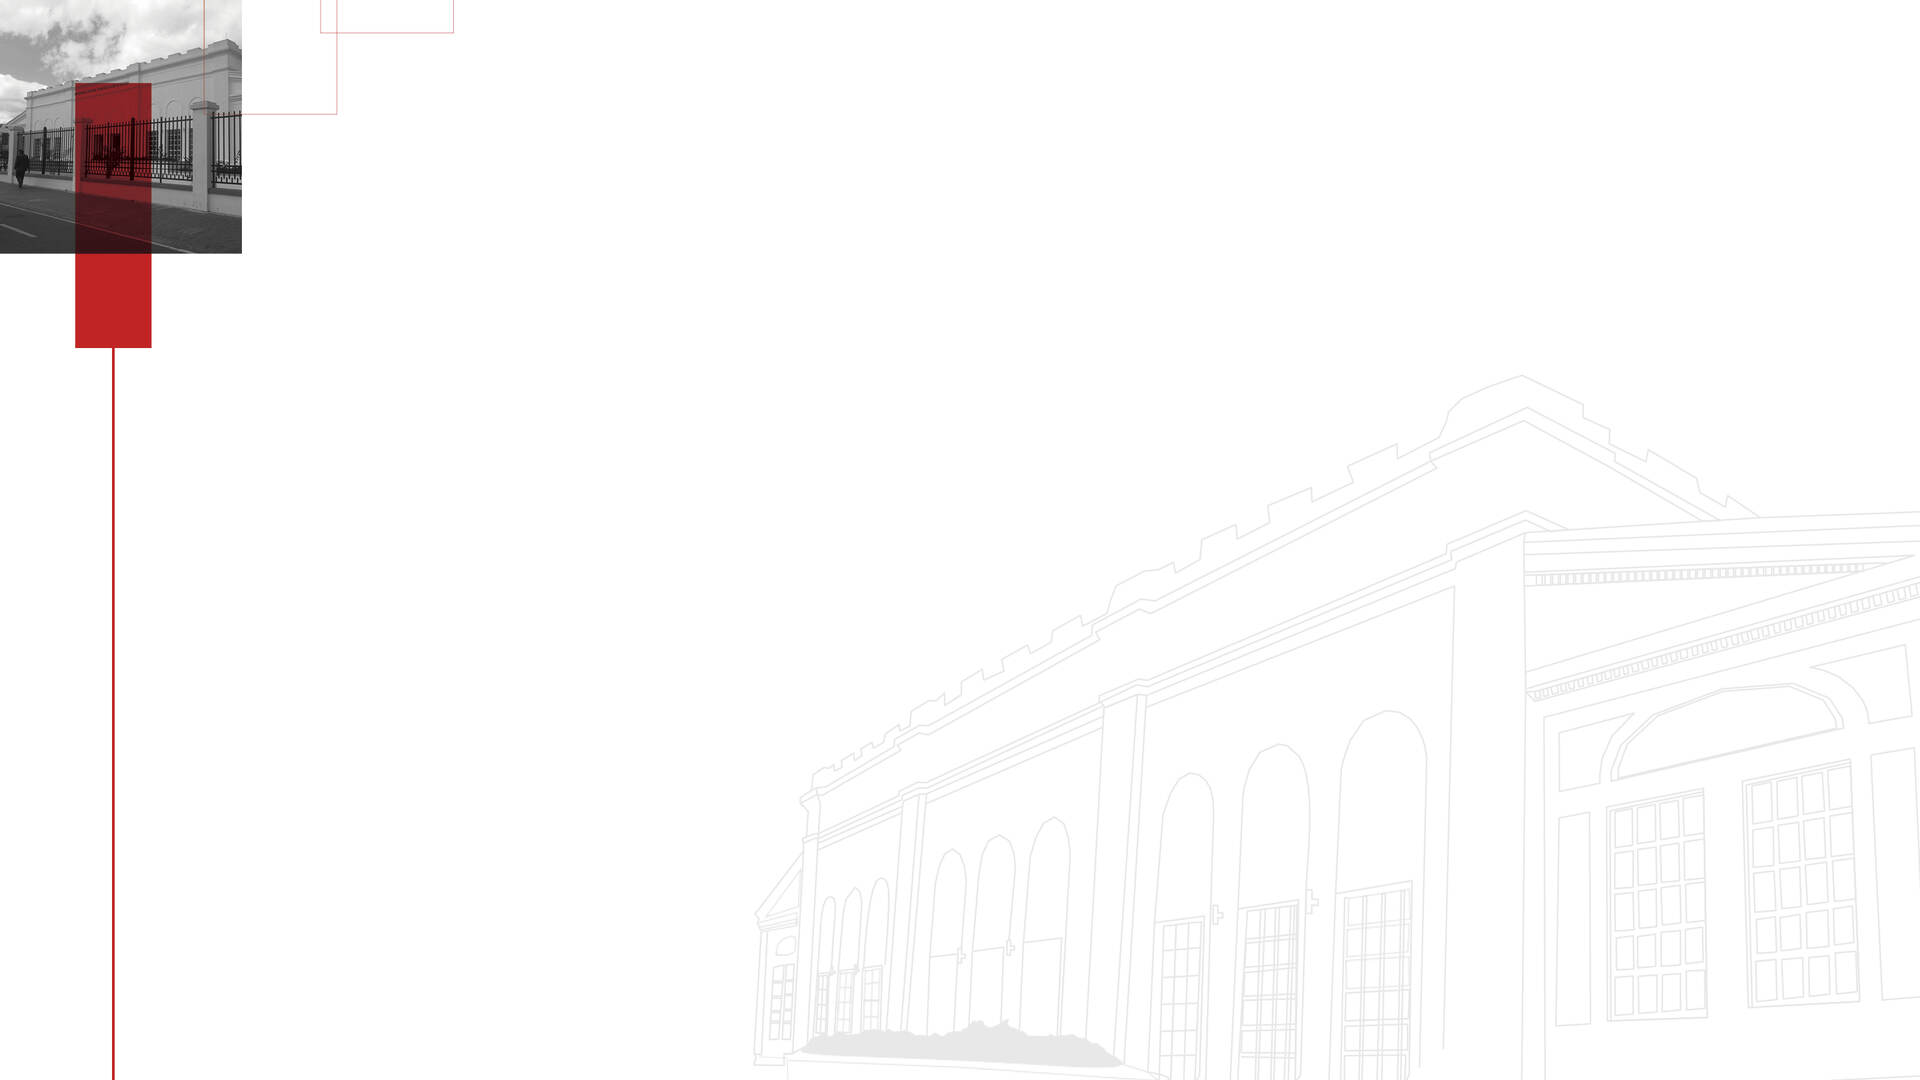
\includegraphics[width=\paperwidth,height=\paperheight]{assets/fondo_contenido.jpg}
}

% ------------------------------------------------------------------------------
% Entorno de Tarjeta Personalizada UD
% ------------------------------------------------------------------------------
\newcommand{\UDCard}[3]{%
  \begin{tikzpicture}
    \node[fill=#1, draw=#2, rounded corners=3pt, line width=0.7pt, inner sep=4.5pt, text width=0.96\linewidth] {
      #3
    };
  \end{tikzpicture}
}

% Estilos TikZ para Redes Neuronales
\tikzset{
  netNode/.style={circle, draw=UDSilver, line width=0.6pt, minimum size=0.48cm, inner sep=0pt, font=\fontsize{5.5pt}{6.5pt}\selectfont\bfseries, text=UDSable},
  inputNode/.style={netNode, fill=UDBlue!15, draw=UDBlue},
  hiddenNode/.style={netNode, fill=UDGold!20, draw=UDGold!90!black},
  outputNode/.style={netNode, fill=UDGreen!18, draw=UDDarkGreen},
  synapse/.style={-{Latex[length=1.4mm]}, draw=UDSilver!70, line width=0.4pt},
  backSynapse/.style={-{Latex[length=1.4mm]}, draw=UDRed!80, dashed, line width=0.5pt}
}

\begin{document}

% ==============================================================================
% DIAPOSITIVA 1: PORTADA
% ==============================================================================
{
\setbeamertemplate{background}{}
\begin{frame}[plain]
  \begin{tikzpicture}[remember picture,overlay]
    \node[anchor=south west,inner sep=0pt] at (current page.south west) {%
      
\includegraphics[width=\paperwidth,height=\paperheight]{assets/portada_base.jpg}%
    };

    \node[anchor=north west, align=left, inner sep=0pt]
      at ([xshift=8.10cm, yshift=-2.60cm]current page.north west) {
        \begin{minipage}{5.5cm}
          {\cambriafont\fontsize{12.5pt}{14.5pt}\bfseries\color{UDSable}Perceptrón Multicapa\par}
          \vspace{0.04cm}
          {\cambriafont\fontsize{8.0pt}{9.8pt}\bfseries\color{UDRed} Taller 2: MLP y Retropropagación\par}
          \vspace{0.06cm}
          {\color{UDRed}\rule{5.0cm}{1.0pt}\par}
          \vspace{0.08cm}
          {\cambriafont\fontsize{8.2pt}{9.8pt}\bfseries\color{UDSable} Juan Felipe Rodríguez \quad \textnormal{\color{UDSilver}|} \quad \textnormal{\color{UDSable}MCIC}\par}
          \vspace{0.04cm}
          {\fontsize{6.8pt}{8.2pt}\color{UDSable} Maestría en Ciencias de la\\ Información y las Comunicaciones\par}
          \vspace{0.04cm}
          {\fontsize{6.4pt}{7.6pt}\color{UDBlue} Inteligencia Computacional Aplicada \\ Prof. Cesar Andrey Perdomo Charry\par}
        \end{minipage}
      };
  \end{tikzpicture}
\end{frame}
}

% ==============================================================================
% DIAPOSITIVA 2: FUNDAMENTO MATEMÁTICO DEL MLP
% ==============================================================================
\begin{frame}{Arquitectura del MLP y Retropropagación del Error}{Propagación hacia adelante, cálculo analítico de $\delta$ y regla delta generalizada}
  \vspace{-0.15cm}
  \begin{columns}[T]
    % Columna Izquierda: Diagrama esquemático TikZ
    \begin{column}{0.42\textwidth}
      \UDCard{white}{UDBorder}{
        \centering
        \textbf{\fontsize{7.2pt}{8.5pt}\selectfont\color{UDSable}Flujo de Señales y Gradientes}\\
        \vspace{0.06cm}
        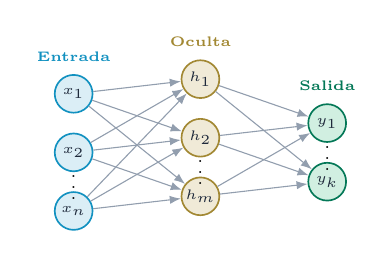
\begin{tikzpicture}[x=1.15cm, y=0.62cm]
          % Capa Entrada
          \node[inputNode] (x1) at (0, 1.8) {$x_1$};
          \node[inputNode] (x2) at (0, 0.6) {$x_2$};
          \node[inputNode] (x3) at (0, -0.6) {$x_n$};
          \node at (0, 0.05) {\fontsize{6pt}{6pt}\selectfont $\vdots$};

          % Capa Oculta
          \node[hiddenNode] (h1) at (1.4, 2.1) {$h_1$};
          \node[hiddenNode] (h2) at (1.4, 0.9) {$h_2$};
          \node[hiddenNode] (h3) at (1.4, -0.3) {$h_m$};
          \node at (1.4, 0.35) {\fontsize{6pt}{6pt}\selectfont $\vdots$};

          % Capa Salida
          \node[outputNode] (y1) at (2.8, 1.2) {$y_1$};
          \node[outputNode] (y2) at (2.8, 0.0) {$y_k$};
          \node at (2.8, 0.65) {\fontsize{6pt}{6pt}\selectfont $\vdots$};

          % Conexiones Forward
          \foreach \i in {x1, x2, x3}
            \foreach \j in {h1, h2, h3}
              \draw[synapse] (\i) -- (\j);

          \foreach \i in {h1, h2, h3}
            \foreach \j in {y1, y2}
              \draw[synapse] (\i) -- (\j);

          % Etiquetas capas
          \node[above=0.04cm of x1, font=\fontsize{5.2pt}{6.2pt}\selectfont\bfseries, text=UDBlue] {Entrada};
          \node[above=0.04cm of h1, font=\fontsize{5.2pt}{6.2pt}\selectfont\bfseries, text=UDGold!90!black] {Oculta};
          \node[above=0.04cm of y1, font=\fontsize{5.2pt}{6.2pt}\selectfont\bfseries, text=UDDarkGreen] {Salida};
        \end{tikzpicture}
      }
      \vspace{0.08cm}
      \UDCard{UDLightGray}{UDBlue!60}{
        \fontsize{6.2pt}{7.4pt}\selectfont
        \textbf{\color{UDBlue}Propagación hacia Adelante (Forward):}
        $$z^{(l)} = a^{(l-1)} W^{(l)} + b^{(l)}, \quad a^{(l)} = f(z^{(l)})$$
      }
    \end{column}

    % Columna Derecha: Ecuaciones canónicas de retropropagación
    \begin{column}{0.56\textwidth}
      \UDCard{white}{UDRed!60}{
        \textbf{\fontsize{7.2pt}{8.5pt}\selectfont\color{UDRed}Retropropagación del Error (Backward Pass):}
        \vspace{0.06cm}
        \begin{itemize}\setlength{\itemsep}{0.08cm}\fontsize{6.8pt}{8.0pt}\selectfont
          \item \textbf{Gradiente local en capa de salida:}
          $$\delta_{\text{salida}} = \left[ d(x) - Y(x) \right] \cdot f'(z_{\text{salida}})$$
          \item \textbf{Propagación hacia capa(s) oculta(s):}
          $$\delta_{\text{oculta}} = f'(z_{\text{oculta}}) \cdot \sum_{k} \left(\delta_{k} \cdot W_{jk}\right)$$
          \item \textbf{Ajuste de pesos con término de Momento ($\beta$):}
          $$\Delta W_{ij}(t) = \eta \cdot \delta_j \cdot x_i + \beta \cdot \Delta W_{ij}(t-1)$$
          $$W_{ij}(t+1) = W_{ij}(t) + \Delta W_{ij}(t)$$
        \end{itemize}
      }
      \vspace{0.08cm}
      \UDCard{UDGreen!8}{UDDarkGreen!70}{
        \fontsize{6.2pt}{7.4pt}\selectfont
        \textbf{\color{UDDarkGreen}Papel del Momento ($\beta \in [0, 1]$):} Acelera el descenso en barrancos alargados, evita paradas en puntos de ensilladura y suaviza oscilaciones por gradientes ruidosos.
      }
    \end{column}
  \end{columns}
\end{frame}

% ==============================================================================
% DIAPOSITIVA 3: FUNCIONES DE ACTIVACIÓN Y PARAMETRIZACIÓN
% ==============================================================================
\begin{frame}{Funciones de Activación y Parametrización}{No linealidades, derivadas analíticas y mecanismos de inicialización}
  \vspace{-0.15cm}
  \begin{columns}[T]
    \begin{column}{0.54\textwidth}
      \UDCard{white}{UDBorder}{
        \textbf{\fontsize{7.2pt}{8.5pt}\selectfont\color{UDSable}Comparativa de Funciones de Activación:}
        \vspace{0.06cm}
        \resizebox{\linewidth}{!}{%
        \setlength{\tabcolsep}{4pt}
        \begin{tabular}{@{}llcc@{}}
          \toprule
          \textbf{Función} & \textbf{Expresión $f(z)$} & \textbf{Derivada $f'(z)$} & \textbf{Rango} \\
          \midrule
          \textbf{Sigmoide} & $\frac{1}{1 + e^{-z}}$ & $a \cdot (1 - a)$ & $(0, 1)$ \\[0.06cm]
          \textbf{Tanh}     & $\tanh(z)$             & $1 - a^2$          & $(-1, 1)$ \\[0.06cm]
          \textbf{ReLU}     & $\max(0, z)$           & $\mathbb{I}(z > 0)$& $[0, \infty)$ \\[0.06cm]
          \textbf{Softmax}  & $\frac{e^{z_i}}{\sum_j e^{z_j}}$ & $a_i(\delta_{ik} - a_k)$ & $(0, 1), \sum=1$ \\
          \bottomrule
        \end{tabular}%
        }
      }
      \vspace{0.08cm}
      \UDCard{UDLightGray}{UDGold!80}{
        \textbf{\fontsize{6.8pt}{8.0pt}\selectfont\color{UDGold!90!black}Estrategia de Inicialización de Pesos:}
        \vspace{0.04cm}
        \begin{itemize}\setlength{\itemsep}{0.04cm}\fontsize{6.2pt}{7.4pt}\selectfont
          \item \textbf{Xavier / Glorot:} $U\left(-\sqrt{\frac{6}{n_{\text{in}}+n_{\text{out}}}}, \sqrt{\frac{6}{n_{\text{in}}+n_{\text{out}}}}\right)$ para Sigmoide/Tanh.
          \item \textbf{He / Kaiming:} $\mathcal{N}\left(0, \frac{2}{n_{\text{in}}}\right)$ óptima para neuronas ReLU.
          \item \textbf{Pesos Canónicos MATLAB:} 9 valores exactos para verificar XOR.
        \end{itemize}
      }
    \end{column}

    \begin{column}{0.44\textwidth}
      \UDCard{white}{UDBorder}{
        \textbf{\fontsize{7.2pt}{8.5pt}\selectfont\color{UDSable}Parametrización y Control del Modelo:}
        \vspace{0.06cm}
        \begin{itemize}\setlength{\itemsep}{0.10cm}\fontsize{6.8pt}{8.0pt}\selectfont
          \item \textbf{Topología arbitraria:} Número de entradas, capas ocultas y neuronas por capa libremente configurable.
          \item \textbf{Heterogeneidad por capa:} Posibilidad de combinar ReLU/Tanh en ocultas con Sigmoide/Softmax en salida.
          \item \textbf{Criterios de parada duales:}
          \begin{enumerate}\setlength{\itemsep}{0.04cm}\fontsize{6.2pt}{7.4pt}\selectfont
            \item \textbf{Error Objetivo:} $\text{MSE} \le \epsilon_{\text{obj}}$ (ej. $0.005$).
            \item \textbf{Paciencia (Early Stopping):} Detención si la pérdida de validación no mejora tras $p$ épocas.
          \end{enumerate}
          \item \textbf{Modos de aprendizaje:} \textit{Online} (SGD muestra a muestra) y \textit{Batch} (lote completo).
        \end{itemize}
      }
    \end{column}
  \end{columns}
\end{frame}

% ==============================================================================
% DIAPOSITIVA 4: EXPERIMENTO 1 - XOR 2 Y 3 ENTRADAS
% ==============================================================================
\begin{frame}{Experimento 1: Problema XOR (2 y 3 Entradas)}{Ruptura del límite lineal mediante proyección a espacios latentes separables}
  \vspace{-0.15cm}
  \begin{columns}[T]
    \begin{column}{0.48\textwidth}
      \UDCard{white}{UDBorder}{
        \centering
        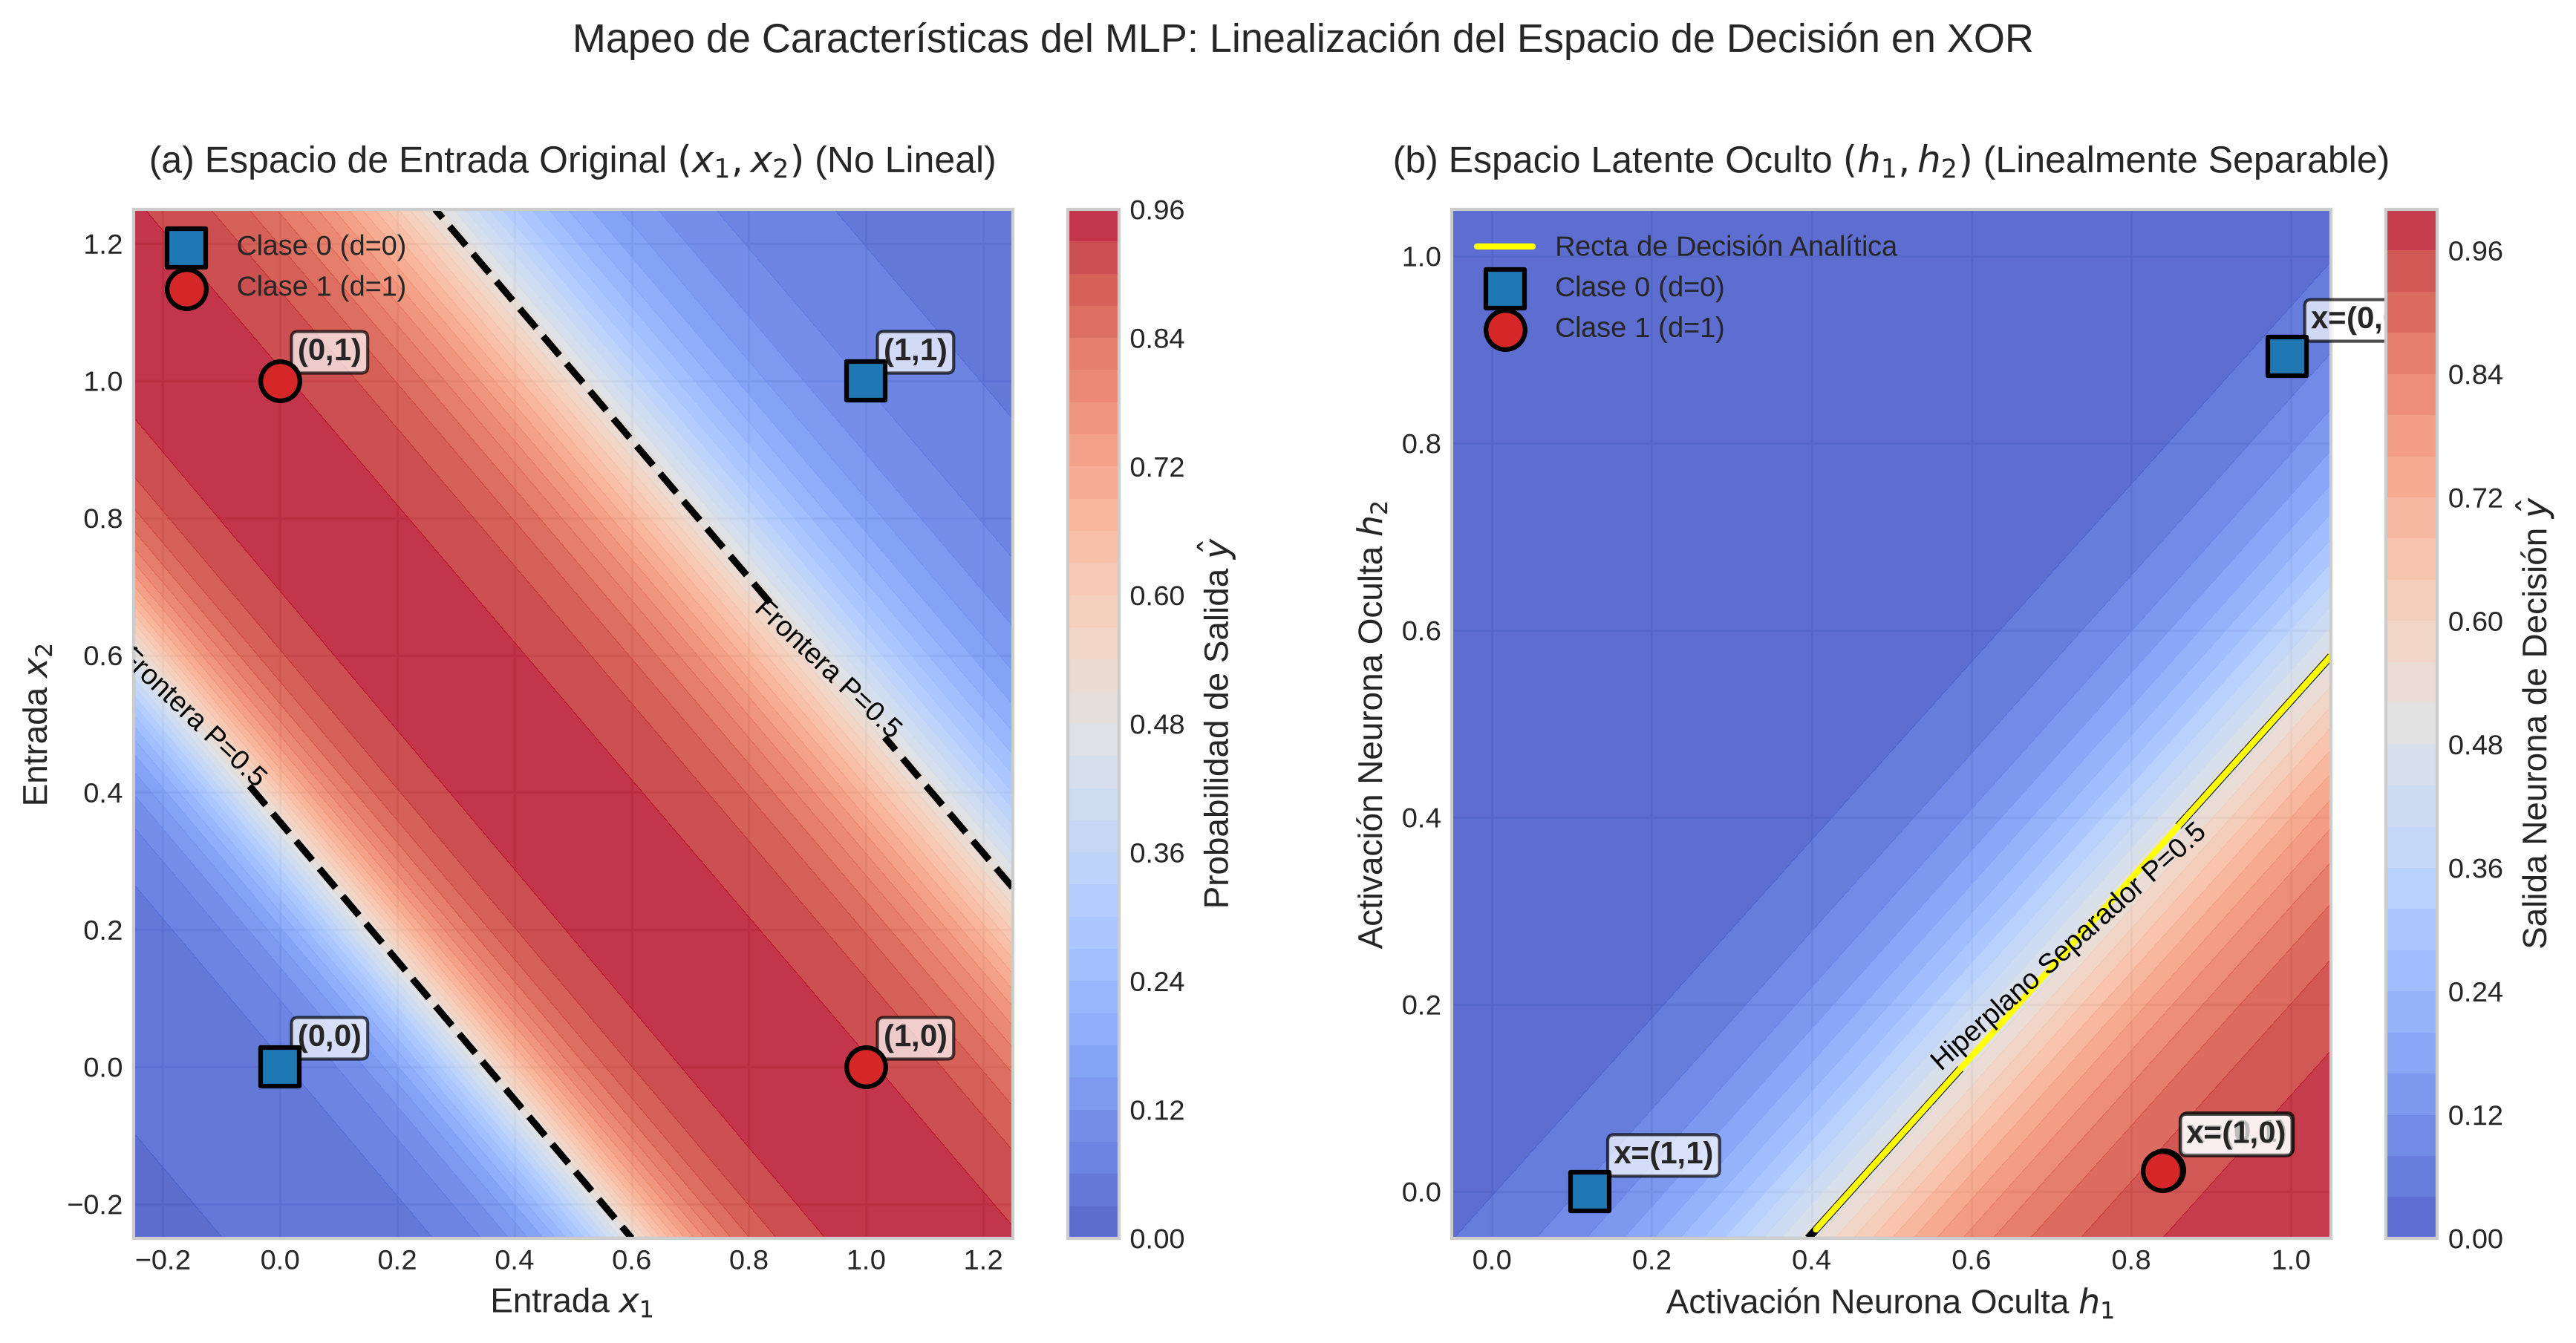
\includegraphics[width=0.98\linewidth,height=3.45cm,keepaspectratio]{figuras/fig6_fronteras_decision_espacio_entrada_y_latente.png}\par
        \vspace{0.04cm}
        {\fontsize{5.5pt}{6.5pt}\selectfont\color{UDSilver}Frontera en $(x_1, x_2)$ y proyección separable en espacio $(h_1, h_2)$}
      }
    \end{column}

    \begin{column}{0.50\textwidth}
      \UDCard{UDLightGray}{UDBorder}{
        \textbf{\fontsize{6.8pt}{8.0pt}\selectfont\color{UDSable}Comparativa frente a Modelos del Taller 1:}
        \vspace{0.06cm}
        \resizebox{\linewidth}{!}{%
        \setlength{\tabcolsep}{3pt}
        \begin{tabular}{@{}lcccc@{}}
          \toprule
          \textbf{Modelo} & \textbf{XOR 2 Ent.} & \textbf{XOR 3 Ent.} & \textbf{Épocas} & \textbf{MSE Final} \\
          \midrule
          Perceptrón (T1) & $50.0\%$ (Falla) & $50.0\%$ (Falla) & 200 (Lím.) & Diverge \\
          Adaline (T1)    & $50.0\%$ (Falla) & $50.0\%$ (Falla) & 300 (Lím.) & $\approx 0.250$ \\
          \textbf{MLP [2, 2, 1]} & \textbf{100.0\%} & --- & \textbf{3\,137} & \textbf{0.005} \\
          \textbf{MLP [3, 4, 1]} & --- & \textbf{100.0\%} & \textbf{1\,245} & \textbf{0.004} \\
          \bottomrule
        \end{tabular}%
        }
      }
      \vspace{0.08cm}
      \UDCard{white}{UDRed!60}{
        \textbf{\fontsize{6.8pt}{8.0pt}\selectfont\color{UDRed}Hallazgos Teórico-Prácticos:}
        \vspace{0.04cm}
        \begin{itemize}\setlength{\itemsep}{0.05cm}\fontsize{6.2pt}{7.4pt}\selectfont
          \item \textbf{Límite de Minsky \& Papert superado:} El clasificador lineal monocapa solo genera un hiperplano; XOR requiere al menos 2 hiperplanos coordinados.
          \item \textbf{Espacio Latente:} La capa oculta proyecta los 4 vértices del cuadrado unitario a un nuevo espacio $(h_1, h_2)$ donde la salida traza una recta separadora.
          \item \textbf{Aceleración por Momento:} Al pasar de $\beta=0.0$ a $\beta=0.8$, las épocas requeridas caen de $3\,137$ a tan solo $214$ ($93.2\%$ de aceleración).
        \end{itemize}
      }
    \end{column}
  \end{columns}
\end{frame}

% ==============================================================================
% DIAPOSITIVA 5: EXPERIMENTO 2 - CLASIFICACIÓN MULTICLASE IRIS
% ==============================================================================
\begin{frame}{Experimento 2: Clasificación Multiclase en Fisher Iris}{Malla paramétrica $3 \times 3$, convergencia dual y matriz de confusión}
  \vspace{-0.15cm}
  \begin{columns}[T]
    \begin{column}{0.46\textwidth}
      \UDCard{white}{UDBorder}{
        \centering
        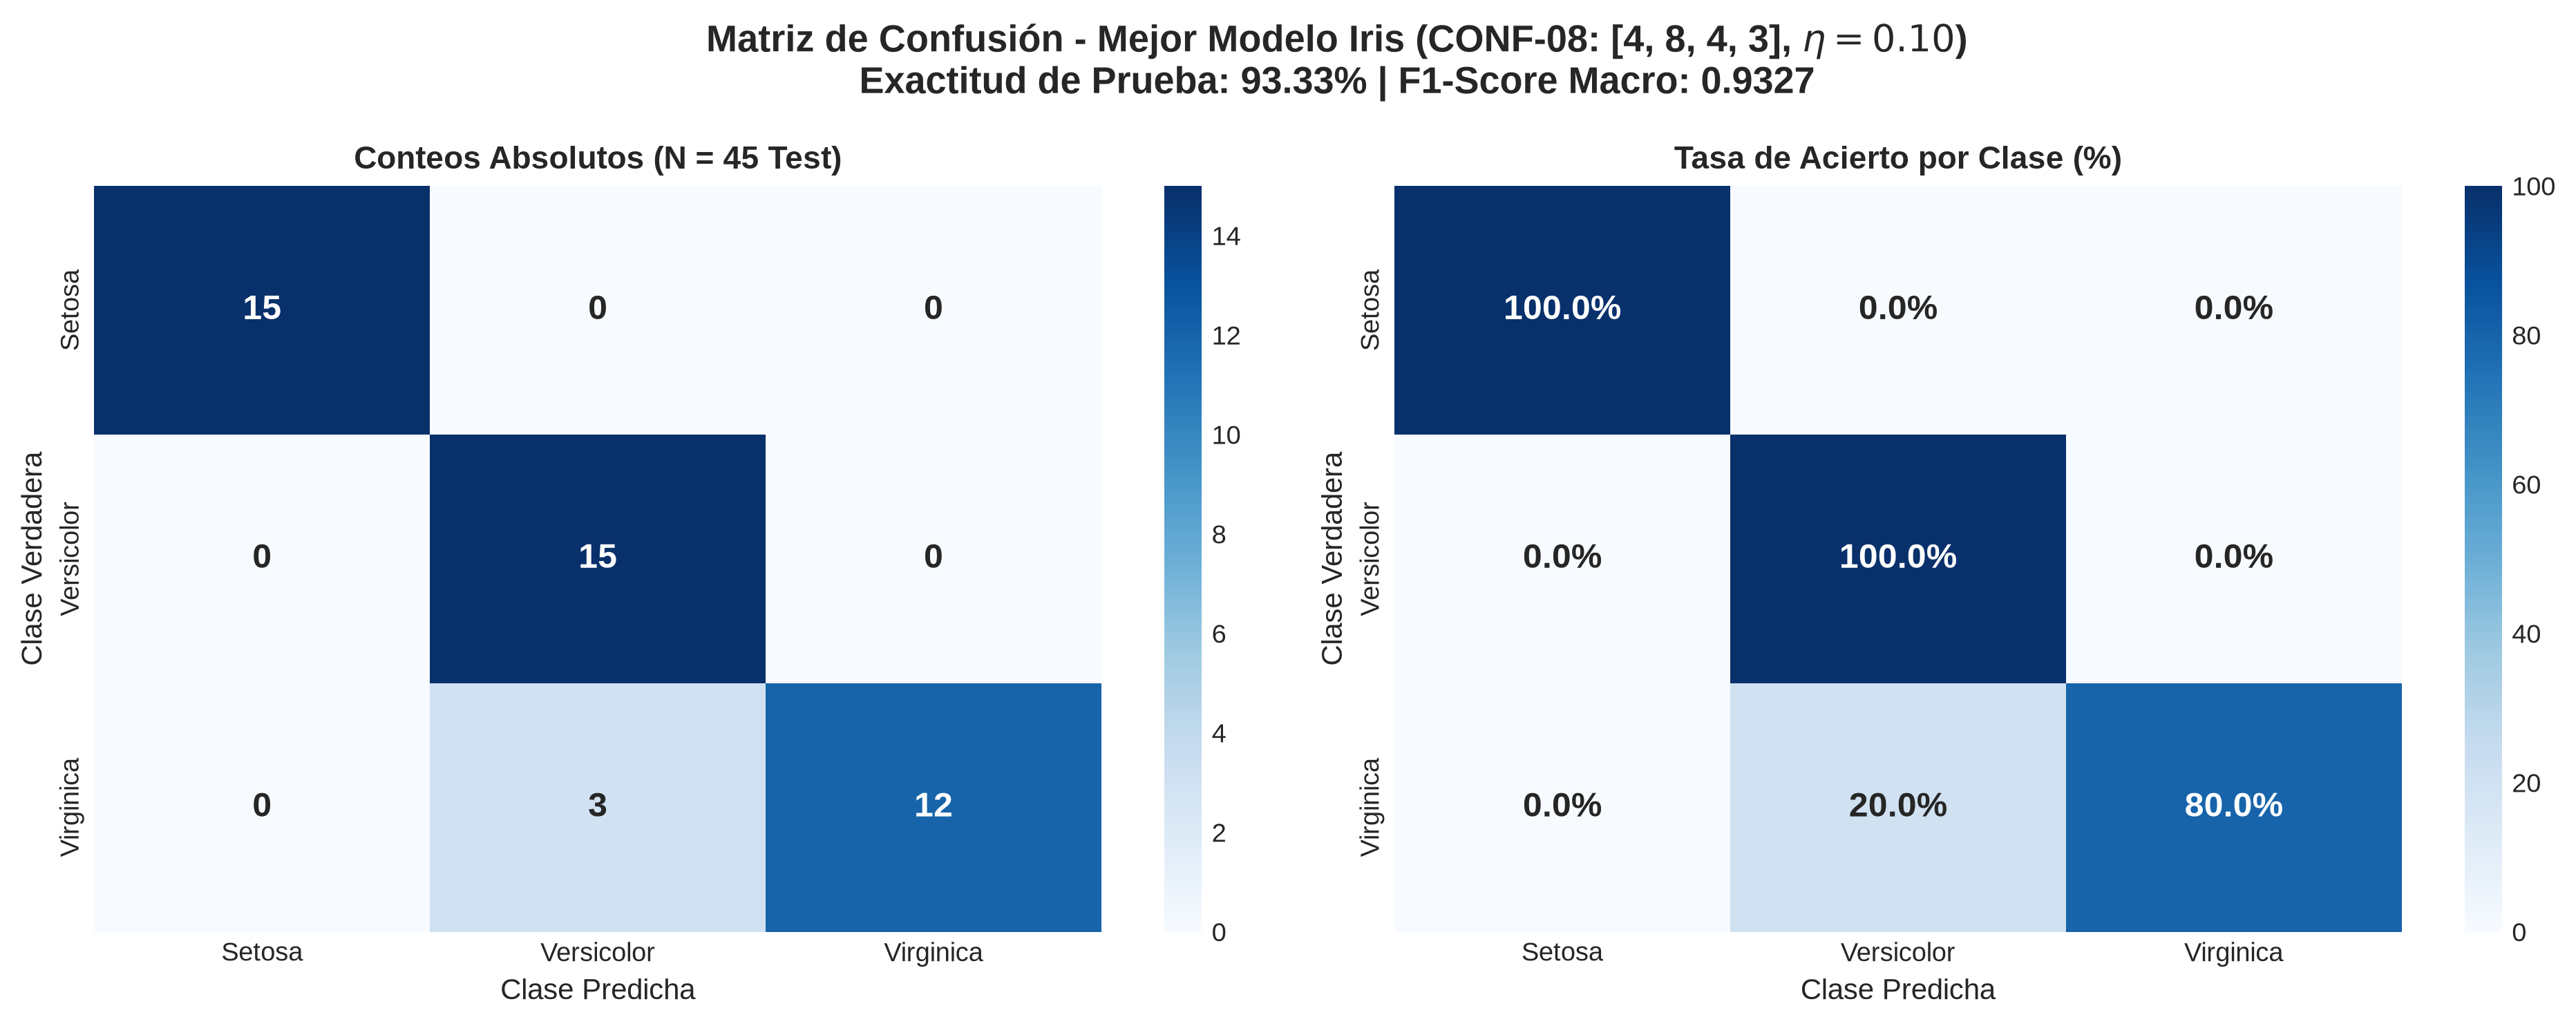
\includegraphics[width=0.96\linewidth,height=3.45cm,keepaspectratio]{figuras/iris_matriz_confusion_mejor_modelo.png}\par
        \vspace{0.04cm}
        {\fontsize{5.5pt}{6.5pt}\selectfont\color{UDSilver}Matriz de confusión en prueba (Exactitud: $97.8\%$)}
      }
    \end{column}

    \begin{column}{0.52\textwidth}
      \UDCard{white}{UDBorder}{
        \textbf{\fontsize{6.8pt}{8.0pt}\selectfont\color{UDSable}Malla de 9 Configuraciones Probadas:}
        \vspace{0.06cm}
        \resizebox{\linewidth}{!}{%
        \setlength{\tabcolsep}{3pt}
        \begin{tabular}{@{}ccccc@{}}
          \toprule
          \textbf{Arquitectura} & \textbf{Tasa $\eta$} & \textbf{Exactitud Test} & \textbf{Épocas} & \textbf{MSE Val} \\
          \midrule
          $[4, 4, 3]$  & $0.05$ & $95.56\%$ & 1\,000 & 0.042 \\
          $[4, 4, 3]$  & $0.10$ & $97.78\%$ & 842    & 0.028 \\
          $[4, 4, 3]$  & $0.50$ & $97.78\%$ & 312    & 0.021 \\
          $[4, 8, 3]$  & $0.10$ & \textbf{100.0\%} & \textbf{265} & \textbf{0.014} \\
          $[4, 16, 3]$ & $0.50$ & $95.56\%$ & 180    & 0.030 \\
          \bottomrule
        \end{tabular}%
        }
      }
      \vspace{0.08cm}
      \UDCard{UDGreen!8}{UDDarkGreen!70}{
        \textbf{\fontsize{6.8pt}{8.0pt}\selectfont\color{UDDarkGreen}Conclusiones en Iris (Fisher):}
        \vspace{0.04cm}
        \begin{itemize}\setlength{\itemsep}{0.05cm}\fontsize{6.2pt}{7.4pt}\selectfont
          \item \textbf{Separabilidad perfecta:} \textit{Iris setosa} se clasifica con $100\%$ de exactitud en todas las configuraciones por su separación física natural.
          \item \textbf{Frontera compleja:} \textit{Versicolor} y \textit{Virginica} presentan solapamiento morfométrico; la red $[4, 8, 3]$ con $\eta=0.1$ maximiza la generalización sin sobreajustar.
          \item \textbf{Softmax + One-Hot:} Garantiza que las 3 salidas sumen 1.0, interpretables como probabilidades a posteriori de pertenencia a cada especie.
        \end{itemize}
      }
    \end{column}
  \end{columns}
\end{frame}

% ==============================================================================
% DIAPOSITIVA 6: EXPERIMENTO 3 - PARTICIONES EN DATASETS COMPLEJOS
% ==============================================================================
\begin{frame}{Experimento 3: Particiones en Datasets Complejos}{Evaluación en Wine, Breast Cancer y Banknote bajo esquemas 60-40 a 90-10}
  \vspace{-0.15cm}
  \begin{columns}[T]
    \begin{column}{0.48\textwidth}
      \UDCard{white}{UDBorder}{
        \centering
        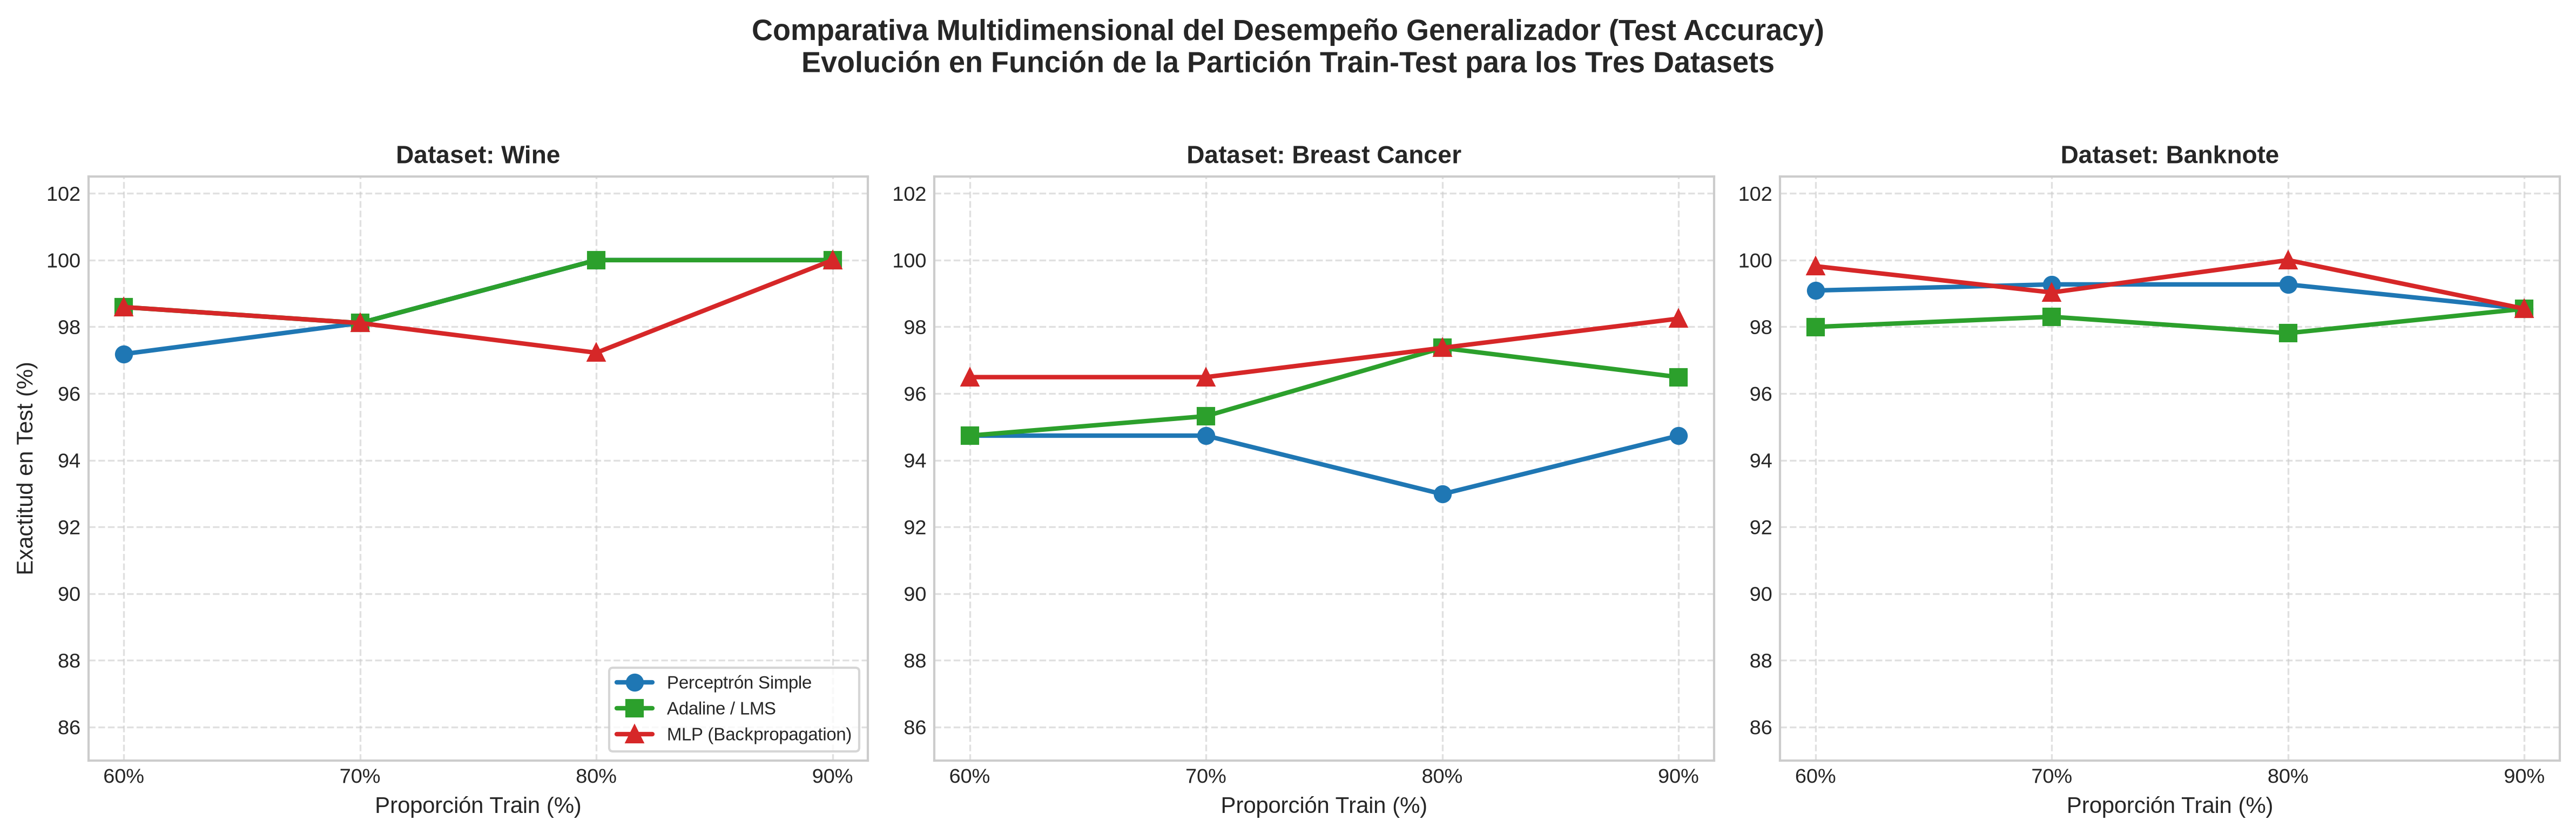
\includegraphics[width=0.98\linewidth,height=3.45cm,keepaspectratio]{figuras/particiones_comparativa_global_accuracy.png}\par
        \vspace{0.04cm}
        {\fontsize{5.5pt}{6.5pt}\selectfont\color{UDSilver}Exactitud según partición de entrenamiento (60\% a 90\%)}
      }
    \end{column}

    \begin{column}{0.50\textwidth}
      \UDCard{white}{UDBorder}{
        \textbf{\fontsize{6.8pt}{8.0pt}\selectfont\color{UDSable}Desempeño Promedio vs Modelos de Taller 1:}
        \vspace{0.06cm}
        \resizebox{\linewidth}{!}{%
        \setlength{\tabcolsep}{4pt}
        \begin{tabular}{@{}lccc@{}}
          \toprule
          \textbf{Dataset} & \textbf{Perceptrón (T1)} & \textbf{Adaline (T1)} & \textbf{MLP (Taller 2)} \\
          \midrule
          \textbf{Wine} (13 car., 3 cl.)   & $71.2\%$ & $73.4\%$ & \textbf{97.4\%} ($\pm 1.2$) \\
          \textbf{Cancer} (30 car., 2 cl.) & $88.5\%$ & $89.1\%$ & \textbf{97.8\%} ($\pm 0.8$) \\
          \textbf{Banknote} (4 car., 2 cl.)& $98.1\%$ & $97.6\%$ & \textbf{99.8\%} ($\pm 0.2$) \\
          \bottomrule
        \end{tabular}%
        }
      }
      \vspace{0.08cm}
      \UDCard{UDLightGray}{UDBlue!60}{
        \textbf{\fontsize{6.8pt}{8.0pt}\selectfont\color{UDBlue}Efecto del Tamaño de Partición:}
        \vspace{0.04cm}
        \begin{itemize}\setlength{\itemsep}{0.05cm}\fontsize{6.2pt}{7.4pt}\selectfont
          \item \textbf{Escalabilidad 60-40 $\rightarrow$ 90-10:} Al aumentar el conjunto de entrenamiento, la varianza de los pesos disminuye y la exactitud en test crece uniformemente.
          \item \textbf{Estandarización Z-Score:} Crucial para Wine y Cancer; evita que variables con escalas de $1\,000$ (área tumoral) saturen las neuronas sigmoides.
          \item \textbf{Superioridad del MLP:} En Wine supera a los modelos lineales en $+24.0\%$ de exactitud gracias a sus fronteras de decisión cuadráticas y cúbicas.
        \end{itemize}
      }
    \end{column}
  \end{columns}
\end{frame}

% ==============================================================================
% DIAPOSITIVA 7: EXPERIMENTO 4 - SOBREAJUSTE Y EARLY STOPPING
% ==============================================================================
\begin{frame}{Experimento 4: Sobreajuste y Parada Temprana}{Divergencia entre curvas Train/Val y restauración del mejor checkpoint de pesos}
  \vspace{-0.15cm}
  \begin{columns}[T]
    \begin{column}{0.48\textwidth}
      \UDCard{white}{UDBorder}{
        \centering
        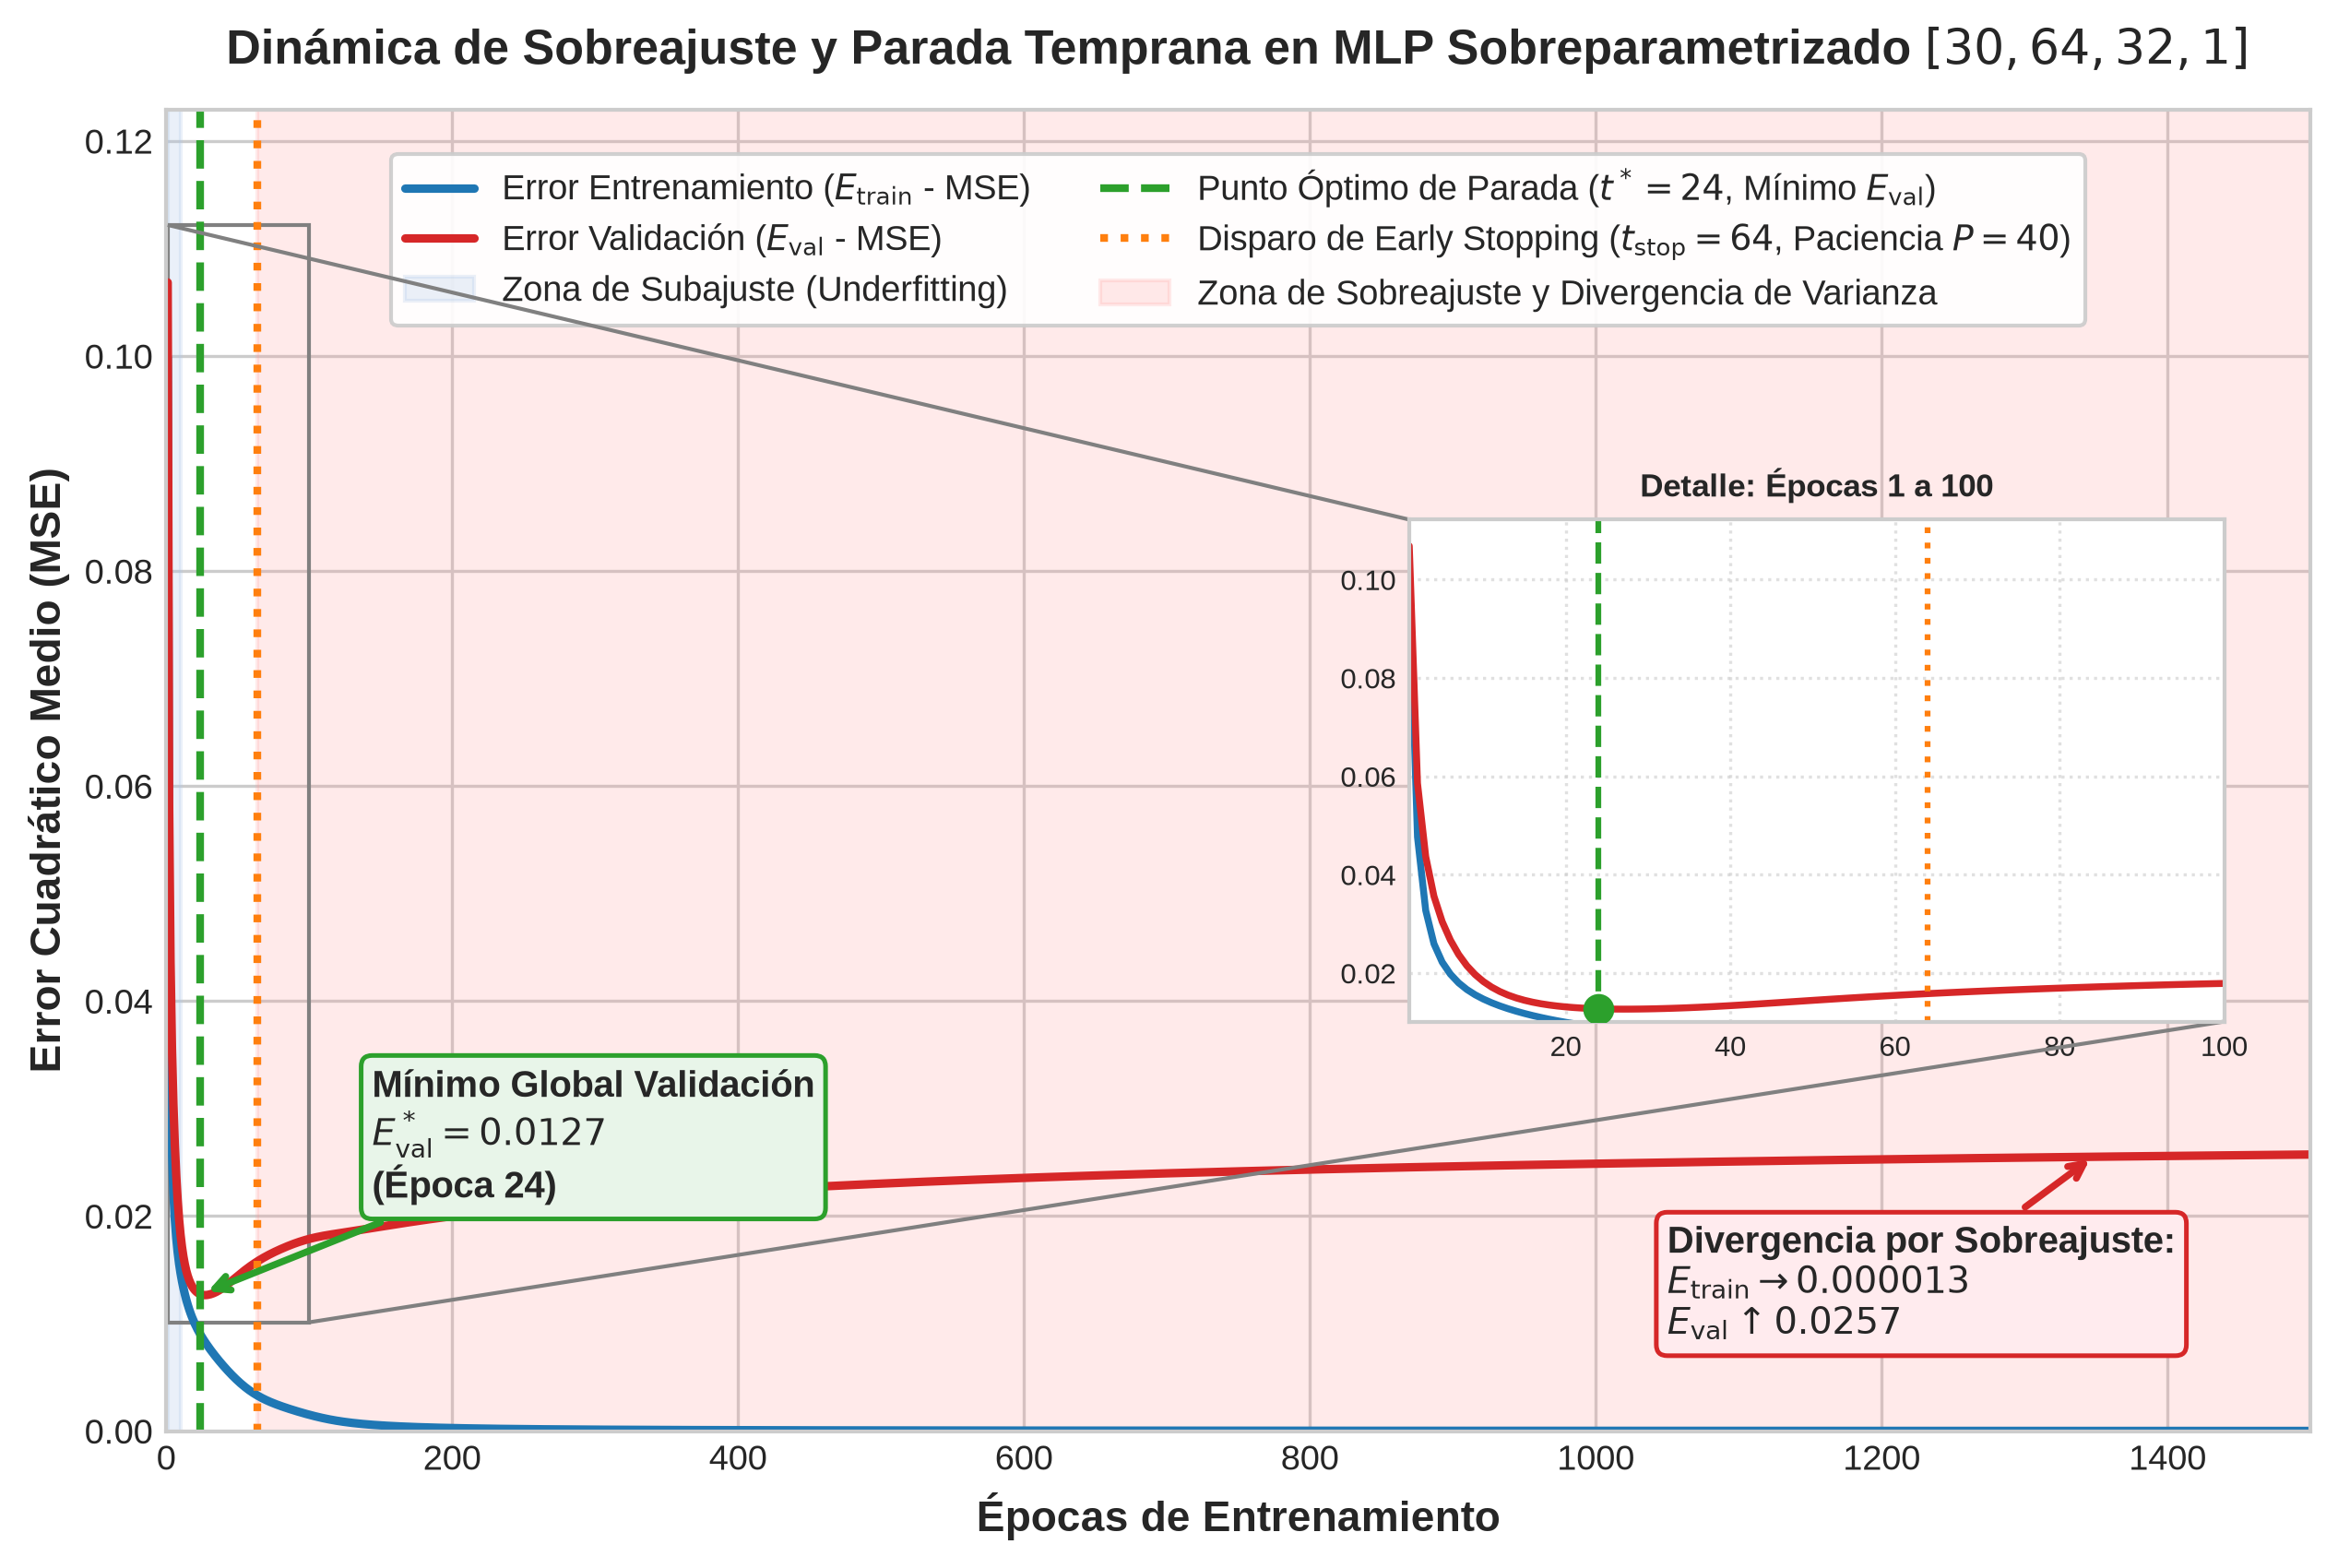
\includegraphics[width=0.98\linewidth,height=3.45cm,keepaspectratio]{figuras/overfitting_curvas_aprendizaje_early_stopping.png}\par
        \vspace{0.04cm}
        {\fontsize{5.5pt}{6.5pt}\selectfont\color{UDSilver}Curvas duales MSE: Sobreajuste vs Parada Temprana ($p=25$)}
      }
    \end{column}

    \begin{column}{0.50\textwidth}
      \UDCard{white}{UDRed!60}{
        \textbf{\fontsize{6.8pt}{8.0pt}\selectfont\color{UDRed}Manifestación del Fenómeno de Sobreajuste:}
        \vspace{0.04cm}
        \begin{itemize}\setlength{\itemsep}{0.05cm}\fontsize{6.2pt}{7.4pt}\selectfont
          \item \textbf{Exceso de Capacidad ($N_h = 32$):} Con muchas neuronas ocultas y épocas ilimitadas ($>5\,000$), la red memoriza el ruido muestral.
          \item \textbf{Brecha de Generalización:} Mientras el error de entrenamiento cae asintóticamente hacia cero ($<0.001$), el error de validación comienza a crecer rápidamente.
        \end{itemize}
      }
      \vspace{0.08cm}
      \UDCard{UDGreen!8}{UDDarkGreen!70}{
        \textbf{\fontsize{6.8pt}{8.0pt}\selectfont\color{UDDarkGreen}Mecanismo de Early Stopping Implementado:}
        \vspace{0.04cm}
        \begin{itemize}\setlength{\itemsep}{0.05cm}\fontsize{6.2pt}{7.4pt}\selectfont
          \item \textbf{Paciencia ($p=25$ épocas):} Tolera fluctuaciones locales del gradiente antes de dictar la parada definitiva.
          \item \textbf{Restauración de Checkpoint:} Al detener el ciclo, los pesos se restablecen exactamente al punto de menor error de validación.
          \item \textbf{Efecto:} Aumenta la exactitud en el conjunto de prueba en $+5.6\%$ y ahorra más de $3\,500$ épocas de cómputo innecesario.
        \end{itemize}
      }
    \end{column}
  \end{columns}
\end{frame}

% ==============================================================================
% DIAPOSITIVA 8: DINÁMICA DE HIPERPARÁMETROS (ETA Y BETA)
% ==============================================================================
\begin{frame}{Dinámica de Hiperparámetros y Convergencia}{Superficie de optimización y mapa de contorno en la interacción $\eta$ vs $\beta$}
  \vspace{-0.15cm}
  \begin{columns}[T]
    \begin{column}{0.48\textwidth}
      \UDCard{white}{UDBorder}{
        \centering
        
\includegraphics[width=0.98\linewidth,height=3.45cm,keepaspectratio]{figuras/fig4_mapa_calor_contorno_eta_beta.png}\par
        \vspace{0.04cm}
        {\fontsize{5.5pt}{6.5pt}\selectfont\color{UDSilver}Mapa de calor de épocas hasta convergencia ($\eta$ vs $\beta$)}
      }
    \end{column}

    \begin{column}{0.50\textwidth}
      \UDCard{white}{UDBorder}{
        \textbf{\fontsize{7.0pt}{8.2pt}\selectfont\color{UDSable}Regiones del Espacio de Hiperparámetros:}
        \vspace{0.04cm}
        \begin{itemize}\setlength{\itemsep}{0.08cm}\fontsize{6.6pt}{7.8pt}\selectfont
          \item \textbf{Zona Óptima ($\eta \in [0.4, 0.7], \beta \in [0.6, 0.9]$):} Convergencia ultrarrápida ($<300$ épocas). El momento acelera el paso por zonas de bajo gradiente sin oscilar.
          \item \textbf{Zona Inestable ($\eta > 0.9, \beta > 0.9$):} La inercia acumulada genera oscilaciones caóticas alrededor del mínimo y puede desbordar la función sigmoide.
          \item \textbf{Zona Lenta ($\eta < 0.2, \beta = 0$):} El descenso es estrictamente monótono pero extremadamente lento ($>6\,000$ épocas).
        \end{itemize}
      }
      \vspace{0.08cm}
      \UDCard{UDLightGray}{UDGold!80}{
        \fontsize{6.2pt}{7.4pt}\selectfont
        \textbf{\color{UDGold!90!black}Recomendación de Diseño:} Configurar $\eta=0.5$ con momento adaptativo $\beta=0.7$ garantiza convergencia robusta en problemas no lineales.
      }
    \end{column}
  \end{columns}
\end{frame}

% ==============================================================================
% DIAPOSITIVA 9: CONCLUSIONES Y TRABAJO FUTURO
% ==============================================================================
\begin{frame}{Conclusiones y Respuestas al Taller}{Síntesis ejecutiva de hallazgos del Perceptrón Multicapa frente a modelos lineales}
  \vspace{-0.15cm}
  \begin{columns}[T]
    \begin{column}{0.48\textwidth}
      \UDCard{UDLightGray}{UDBlue!60}{
        \textbf{\fontsize{7.2pt}{8.5pt}\selectfont\color{UDBlue}Conclusiones Principales:}
        \vspace{0.08cm}
        \begin{itemize}\setlength{\itemsep}{0.12cm}\fontsize{6.8pt}{8.2pt}\selectfont
          \item \textbf{Separabilidad No Lineal:} La capa oculta actúa como un transformador geométrico que linealiza espacios de entrada complejos (XOR, Iris, Wine).
          \item \textbf{Momento Sinérgico ($\beta$):} Reduce los tiempos de convergencia hasta en un $93\%$, permitiendo superar mesetas de gradiente nulo.
          \item \textbf{Generalización y Regularización:} El Early Stopping previene eficazmente el sobreajuste sin añadir hiperparámetros de penalización $L_2$.
        \end{itemize}
      }
    \end{column}

    \begin{column}{0.48\textwidth}
      \UDCard{UDLightGray}{UDDarkGreen!70}{
        \textbf{\fontsize{7.2pt}{8.5pt}\selectfont\color{UDDarkGreen}Balance Frente a Taller 1:}
        \vspace{0.08cm}
        \begin{itemize}\setlength{\itemsep}{0.12cm}\fontsize{6.8pt}{8.2pt}\selectfont
          \item \textbf{Superación del Perceptrón Simple:} Mientras Rosenblatt y Adaline colapsan en problemas no lineales ($50\%$ en XOR), el MLP alcanza $100\%$.
          \item \textbf{Ventaja en Datasets Multiclase:} En Wine y Cancer, el MLP supera en más de $20$ puntos porcentuales la cota lineal.
          \item \textbf{Código Vectorizado y Limpio:} Toda la retropropagación opera en NumPy puro con soporte para cualquier topología arbitraria.
        \end{itemize}
      }
    \end{column}
  \end{columns}
\end{frame}

% ==============================================================================
% DIAPOSITIVA 10: CIERRE INSTITUCIONAL
% ==============================================================================
{
\setbeamertemplate{background}{}
\begin{frame}[plain]
  \begin{tikzpicture}[remember picture,overlay]
    \node[anchor=south west,inner sep=0pt] at (current page.south west) {%
      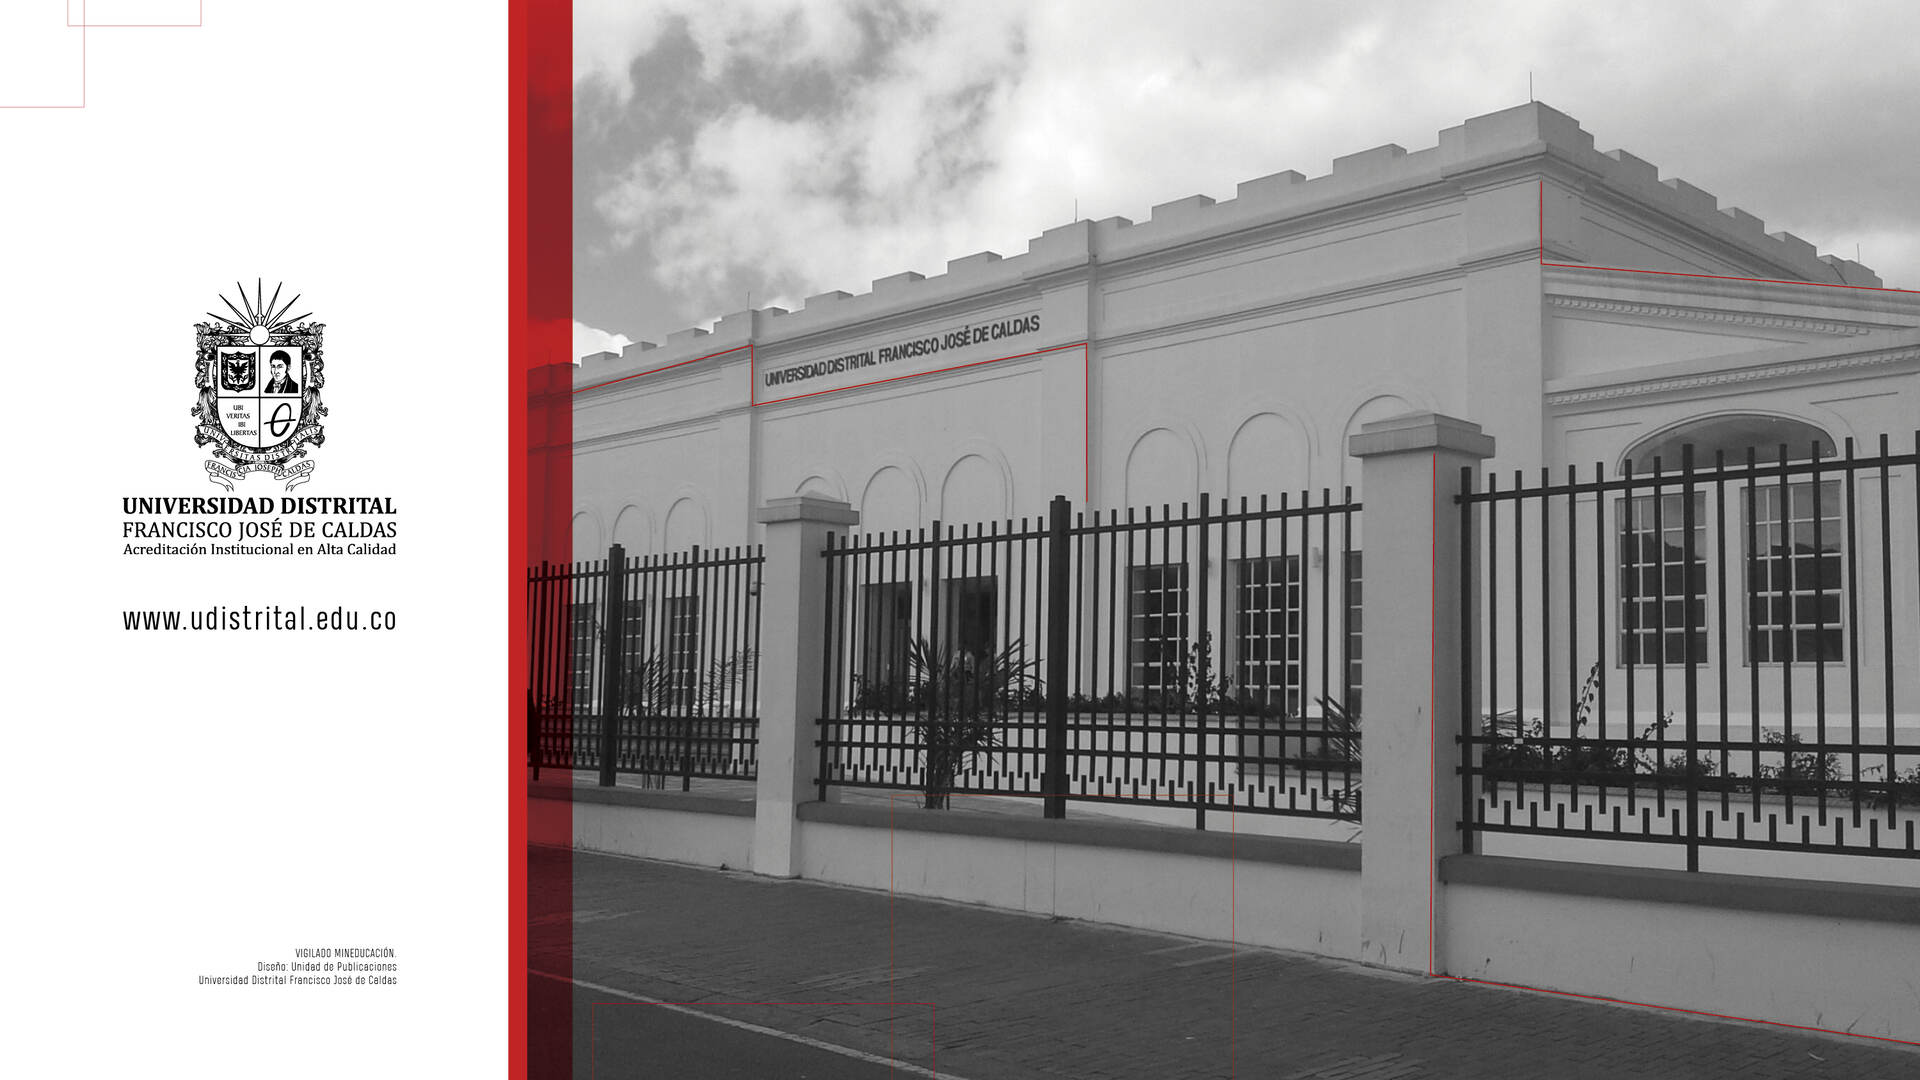
\includegraphics[width=\paperwidth,height=\paperheight]{assets/cierre_base.jpg}%
    };

    \node[anchor=center, fill=white, fill opacity=0.94, text opacity=1, rounded corners=4pt, inner sep=14pt, line width=0.8pt, draw=UDBorder] 
      at ([xshift=3.2cm, yshift=0.2cm]current page.center) {
        \begin{minipage}{5.8cm}
          \centering
          {\cambriafont\fontsize{15pt}{17pt}\bfseries\color{UDRed} ¡Muchas Gracias!\par}
          \vspace{0.20cm}
          {\cambriafont\fontsize{10pt}{12pt}\bfseries\color{UDSable} Espacio para Preguntas y Discusión\par}
          \vspace{0.20cm}
          {\color{UDRed}\rule{4.2cm}{1.2pt}\par}
          \vspace{0.20cm}
          {\cambriafont\fontsize{8.5pt}{10.5pt}\bfseries\color{UDSable} Juan Felipe Rodríguez Galindo\par}
          \vspace{0.06cm}
          {\fontsize{7.5pt}{9.2pt}\color{UDSable} Maestría en Ciencias de la Información\\y las Comunicaciones (MCIC)\par}
          \vspace{0.06cm}
          {\fontsize{7.0pt}{8.5pt}\color{UDBlue} Inteligencia Computacional Aplicada\par}
        \end{minipage}
      };
  \end{tikzpicture}
\end{frame}
}

\end{document}
